\documentclass[slidestop,mathserif,compress,xcolor=svgnames]{beamer} 
\mode<presentation>
{  
  \setbeamertemplate{background canvas}[vertical shading][bottom=blue!5,top=blue!5]
  \setbeamertemplate{navigation symbols}{}%{\insertsectionnavigationsymbol}
    \usetheme{LSU}
%  default infolines miniframes shadow sidebar smoothbars smoothtree split tree
%    \useoutertheme{shadow}
}

\usepackage{pgf,pgfarrows,pgfnodes,pgfautomata,pgfheaps,pgfshade}
\usepackage{amsmath,amssymb,amsfonts,subfigure}
\usepackage{tabularx}
\usepackage{booktabs}
\usepackage{colortbl}
\usepackage{tikz}
\usetikzlibrary{shapes,arrows}
\usetikzlibrary{calc}
\pgfdeclarelayer{background}
\pgfdeclarelayer{foreground}
\pgfsetlayers{background,main,foreground}
\usepackage[latin1]{inputenc}
\usepackage{colortbl}
\usepackage[english]{babel}
\usepackage{hyperref}
\usepackage[normalem]{ulem}
% \usepackage{movie15}
\hypersetup{
  pdftitle={Electronic Structure Calculation in Quantum Chemistry},
  pdfauthor={Alexander B. Pacheco, User Services Consultant, Louisiana State University}
}
%\usepackage{movie15}
\usepackage{times}

\setbeamercovered{dynamic}
\beamersetaveragebackground{DarkBlue!2}
\beamertemplateballitem

\usepackage[english]{babel}
\usepackage[latin1]{inputenc}
\usepackage{times}
\usepackage{amsmath}
\usepackage[T1]{fontenc}
\usepackage{graphicx}
\definecolor{DarkGreen}{rgb}{0.0,0.3,0.0}
\definecolor{darkgreen}{rgb}{0.0,0.6,0.0}
\definecolor{Blue}{rgb}{0.0,0.0,0.8} 
\definecolor{dodgerblue}{rgb}{0.1,0.1,1.0}
\definecolor{indigo}{rgb}{0.41,0.1,0.0}
\definecolor{seagreen}{rgb}{0.1,1.0,0.1}
\DeclareSymbolFont{extraup}{U}{zavm}{m}{n}
\DeclareMathSymbol{\vardiamond}{\mathalpha}{extraup}{87}
\newcommand*\up{\textcolor{green}{%
  \ensuremath{\blacktriangle}}}
\newcommand*\down{\textcolor{red}{%
  \ensuremath{\blacktriangledown}}}
\newcommand*\const{\textcolor{darkgray}%
  {\textbf{--}}}

\setbeamercolor{uppercol}{fg=white,bg=red!30!black}%
\setbeamercolor{lowercol}{fg=black,bg=red!15!white}%
\setbeamercolor{uppercol1}{fg=white,bg=blue!30!black}%
\setbeamercolor{lowercol1}{fg=black,bg=blue!15!white}%%
\setbeamercolor{uppercol2}{fg=white,bg=green!30!black}%
\setbeamercolor{lowercol2}{fg=black,bg=green!15!white}%
\newenvironment{colorblock}[4]
{
\setbeamercolor{upperblock}{fg=#1,bg=#2}
\setbeamercolor{lowerblock}{fg=#3,bg=#4}
\begin{beamerboxesrounded}[upper=upperblock,lower=lowerblock,shadow=true]}
{\end{beamerboxesrounded}}
\newenvironment{ablock}[0]
{
\begin{beamerboxesrounded}[upper=uppercol,lower=lowercol,shadow=true]}
{\end{beamerboxesrounded}}
\newenvironment{bblock}[0]
{
\begin{beamerboxesrounded}[upper=uppercol1,lower=lowercol1,shadow=true]}
{\end{beamerboxesrounded}}
\newenvironment{eblock}[0]
{
\begin{beamerboxesrounded}[upper=uppercol2,lower=lowercol2,shadow=true]}
{\end{beamerboxesrounded}}

\title[Electronic Structure]{Electronic Structure Calculations in Quantum Chemistry}


\author[Alex Pacheco]{\large{Alexander~B.~Pacheco}}
       
\institute[HPC@LSU - http://www.hpc.lsu.edu] {\inst{}\footnotesize{User Services Consultant\\LSU HPC \& LONI\\sys-help@loni.org}}

\date[{Nov 11, 2011\hspace{2cm}}]{\scriptsize{HPC Training\\Louisiana State University\\Baton Rouge\\Nov 16, 2011}}
     
\subject{Talks}
% This is only inserted into the PDF information catalog. Can be left
% out. 




% If you have a file called "university-logo-filename.xxx", where xxx
% is a graphic format that can be processed by latex or pdflatex,
% resp., then you can add a logo as follows:

% Main Logo on bottom left
\pgfdeclareimage[height=0.55cm]{its-logo}{PUR_BLK_HOR}
\logo{\pgfuseimage{its-logo}}
% University Logo on top left
\pgfdeclareimage[height=0.55cm]{university-logo}{LSUGeauxPurp}
\tllogo{\pgfuseimage{university-logo}}
% Logo at top right
\pgfdeclareimage[height=0.6cm]{institute-logo}{LONI}
\trlogo{\pgfuseimage{institute-logo}}
% Logo at bottom right
\pgfdeclareimage[height=0.55cm]{hpc-logo}{LONI-2}
\brlogo{\pgfuseimage{hpc-logo}}


% Delete this, if you do not want the table of contents to pop up at
% the beginning of each subsection:
%  \AtBeginSection[]
%  {
%    \begin{frame}<beamer>
%     \frametitle{\small{Outline}}
%      \small
%      \tableofcontents[currentsection,currentsubsection]
%    \end{frame}
%  }

\begin{document}
\footnotesize

\frame{\titlepage}

\begin{frame}[label=toc,squeeze]
  \footnotesize
  \frametitle{\small{Outline}}
  \tableofcontents
\end{frame}


%\part{Introduction}
\section{Introduction}
\begin{frame}
 \frametitle{\small Introduction}
  \begin{block}{{\bf What is Computational Chemistry?}}
    \begin{itemize}
      \item {\bf Computational Chemistry} is a branch of chemistry that uses computer science to assist in solving chemical problems.
      \item Incorporates the results of theoretical chemistry into efficient computer programs.
      \item Application to single molecule, groups of molecules, liquids or solids.
      \item Calculates the structure and properties of interest.
      \item Computational Chemistry Methods range from
      \begin{enumerate}
	\footnotesize{
	\item Highly accurate ({\it Ab-initio},DFT) feasible for small systems
	\item Less accurate (semi-empirical)
	\item Very Approximate (Molecular Mechanics) large systems
	}
      \end{enumerate}
     \end{itemize}
  \end{block}
\end{frame}

\begin{frame}
 \frametitle{\small Introduction}
  \begin{columns}
    \column{11cm}
    \begin{exampleblock}{{\bf Theoretical Chemistry can be broadly divided into two main categories}}
      \begin{enumerate}
	\item Static Methods {\Large$\Rightarrow$} {\color{blue}Time-Independent Schr\"{o}dinger Equation}
	\begin{enumerate}
	  \footnotesize{
	  \item[]{\Large\hspace{3cm}${\color{DarkGreen}\hat{H}\Psi=E\Psi}$}
	  \item[] 
	  \item[$\vardiamond$] Quantum Chemical/\emph{Ab Initio} /Electronic Structure Methods
	  \item[$\vardiamond$] Molecular Mechanics
	  }
	\end{enumerate}
	\item Dynamical Methods {\Large$\Rightarrow$} {\color{blue}Time-Dependent Schr\"{o}dinger Equation}
	\begin{enumerate}
	  \footnotesize{
	  \item[]{\Large\hspace{3cm}${\color{DarkGreen}\imath\hbar\dfrac{\partial}{\partial t}\Psi = \hat{H}\Psi}$}
	  \item[] 
	  \item[$\vardiamond$] Classical Molecular Dynamics
	  \item[$\vardiamond$] Semi-classical and \textit{Ab-Initio} Molecular Dynamics
	  }
	\end{enumerate}
      \end{enumerate}
    \end{exampleblock}
  \end{columns}
\end{frame}

\begin{frame}
  \frametitle{\small Tutorial Goals}
  \begin{itemize}
    \item Provide a brief introduction to Electronic Structure Calculations in Quantum Chemistry.
    \begin{enumerate}
      \item Overview of Quantum Chemical methods.
      \item What kind of calculations can we carry out?
      \item What experimental properties can we study/understand?
      \item How to create input files?
      \item Tips and Tricks to run calculations?
    \end{enumerate}
  \end{itemize}
\end{frame}


%\part{Ab initio Methods}
\section{Ab Initio Methods}
\begin{frame}
  \frametitle{\small Ab Initio Methods}
  \begin{block}{}
    \begin{itemize}
      \item \emph{Ab Initio}, meaning "from first principles", methods solve the Schr\"{o}dinger equation and does not rely on empirical or experimental data. 
      \item Begining with fundamental and physical properties, calculate how electrons and nuclei interact.
      \item The Schr\"{o}dinger equation can be solved exactly only for a few systems
      \begin{itemize}
	\footnotesize{
	\item[$\vardiamond$] Particle in a Box
	\item[$\vardiamond$] Rigid Rotor
	\item[$\vardiamond$] Harmonic Oscillator
	\item[$\vardiamond$] Hydrogen Atom
	}
      \end{itemize}
      \item For complex systems, \emph{Ab Initio} methods make assumptions to obtain approximate solutions to the  Schr\"{o}dinger equations and solve it numerically.
      \item "Computational Cost" of calculations increases with the accuracy of the calculation and size of the system.
    \end{itemize}
  \end{block}
\end{frame}

\begin{frame}
%   \frametitle{\small Ab Initio Methods}
  \fontsize{9}{10}{
  \vspace{-0.1cm}
  \begin{block}{What can we predict with \emph{Ab Initio} methods?}
    \begin{itemize}
      \item Molecular Geometry: Equilibrium and Transition State
      \item Dipole and Quadrupole Moments and polarizabilities
      \item Thermochemical data like Free Energy, Energy of reaction.
      \item Potential Energy surfaces, Barrier heights
      \item Reaction Rates and cross sections
      \item Ionization potentials (photoelectron and X-ray spectra) and Electron affinities
      \item Frank-Condon factors (transition probabilities, vibronic intensities)
      \item Vibrational Frequencies, IR and Raman Spectra and Intensities
      \item Rotational spectra
      \item NMR Spectra
      \item Electronic excitations and UV-VIS spectra
      \item Electron density maps and population analyses
      \item Thermodynamic quantities like partition function
    \end{itemize}
  \end{block}
  }
\end{frame}


\begin{frame}
  %\frametitle{\small Ab Initio Methods}
  \begin{block}{Ab Initio Theory}
    \begin{itemize}
      \item {\color{blue}Born-Oppenheimer Approximation}: Nuclei are heavier than electrons and can be considered stationary with respect to electrons. Also know as "clamped nuclei" approximations and leads to idea of potential surface
      \item {\color{blue}Slater Determinants}: Expand the many electron wave function in terms of Slater determinants.
      \item {\color{blue}Basis Sets}: Represent Slater determinants by molecular orbitals, which are linear combination of atomic-like-orbital functions i.e. basis sets
    \end{itemize}
  \end{block}
\end{frame}

\begin{frame}
  \frametitle{\small Born-Oppenheimer Approximation}
  \begin{block}{}
    \begin{itemize}
      \item Solve time-independent Schr\"{o}dinger equation
%       \begin{align*}
      \item[]\hspace{4cm}$\hat{H}\Psi = E\Psi$
%       \end{align*}
      \item For many electron system:
%       \begin{align*}
      \item[]\hspace{-0.5cm}$\displaystyle{\hat{H} = -{\color{DarkGreen}\underbrace{\frac{\hbar^2}{2}\sum_\alpha\frac{\nabla^2_\alpha}{M_\alpha}}_{\hat{T}_n}} - {\color{darkgreen}\underbrace{\frac{\hbar^2}{2m_e}\sum_i\nabla^2_i}_{\hat{T}_e}} + {\color{dodgerblue}\underbrace{{\color{Blue}\underbrace{\sum_{\alpha>\beta}\frac{e^2Z_{\alpha}Z_{\beta}}{4\pi\epsilon_0R_{\alpha\beta}}}_{\hat{V}_{nn}}} - {\color{indigo}\underbrace{\sum_{\alpha,i}\frac{e^2Z_{\alpha}}{4\pi\epsilon_0R_{\alpha i}}}_{\hat{V}_{en}}} + {\color{red}\underbrace{\sum_{i>j}\frac{e^2}{4\pi\epsilon_0r_{ij}}}_{\hat{V}_{ee}}}}_{\hat{V}}}}$
%       \end{align*}
      \item The wave function $\Psi(R,r)$ of the many electron molecule is a function of nuclear ($R$) and electronic ($r$) coordinates.
      \item Motion of nuclei and electrons are coupled.
      \item However, since nuclei are much heavier than electrons, the nuclei appear fixed or stationary.
    \end{itemize}
  \end{block}
\end{frame}

\begin{frame}
  \frametitle{\small Born-Oppenheimer Approximation}
  \begin{itemize}
    \item Born-Oppenheimer Approximation: Separate electronic and nuclear motion:
    \begin{align*}
      \Psi(R,r) = \psi_e(r;R)\psi_n(R)
    \end{align*}
    \item Solve electronic part of Schr\"{o}dinger equation
    \begin{align*}
      \hat{H}_e\psi_e(r;R) = E_e\psi_e(r;R)
    \end{align*}
  \end{itemize}
  \begin{columns}
    \column{5cm}
    \vspace{-0.5cm}
    \begin{itemize}
      \item BO approximation leads to the concept of potential energy surface
      \begin{align*}
	V(R) = E_e + V_{nn}
      \end{align*}
      \item The electronic potential is a function of nuclear coordinates.
      \item In Molecular Dynamics, the nuclei move along this energy surface obeying Newton's Laws of Motion.
    \end{itemize}
    \column{6cm}
    \vspace{-0.5cm}
    \begin{exampleblock}{}
      \includegraphics[width=6cm,keepaspectratio=true,clip=true]{HOH}
    \end{exampleblock}
  \end{columns}
\end{frame}

\begin{frame}
  \frametitle{\small Potential Energy Surfaces}
  \begin{itemize}
    \item The potential energy surface (PES) is multi-dimensional ($3N-6$ for non-linear molecule and $3N-5$ for linear molecule)
    \item The PES contains multiple minima and maxima.\let\thefootnote\relax\footnotetext{\tiny Picture taken from Bernard Schlegel's course slide at http://www.chem.wayne.edu/$\sim$hbs/chm6440/}
    \item Geometry optimization search aims to find the global minimum of the potential surface.
    \item Transition state or saddle point search aims to find the maximum of this potential surface, usually along the reaction coordinate of interest.
  \end{itemize}
  \begin{center}
    \includegraphics[width=6cm,keepaspectratio=true,clip=true]{PES}
  \end{center}
\end{frame}

\begin{frame}
  \frametitle{\small Geometry Optimizations}
  \vspace{-0.6cm}
  {\scriptsize
  \begin{columns}
    \column{12cm}
    \begin{block}{}
      \begin{itemize}
	\item Geometry optimization is used to find minima on the potential energy surface, with these minimum energy structures representing equilibrium structures. 
	\item Optimization also is used to locate transition structures, which are represented by saddle points on the potential energy surface. 
	\item Optimization to minima is also referred to as energy minimization. 
	\item During minimization, the energy of molecules is reduced by adjusting atomic coordinates.% It is applied to model-built structures as well as to those derived from coordinate data banks. 
	\item Energy minimization is done when using either molecular mechanics or quantum mechanics methods, and it must precede any computational analyses in which these methods are applied. 
	\item For example, geometry optimization can be used to
	\begin{enumerate}
	  {\scriptsize
	  \item characterize a potential energy surface
	  \item obtain a structure for a single-point quantum mechanical calculation, which provides a large set of structural and electronic properties
	  \item prepare a structure for molecular dynamics simulation - if the forces on atoms are too large, the integration algorithm may fail.
	  }
	\end{enumerate}
	%\item The energy obtained from the potential energy function at the optimized geometry is sometimes called a steric or conformational energy. %These energies can be used to calculate differences between stereoisomers and between isologous molecules (i.e., those differing in connectivity but having the same number of each type of functional group). 
	\item These energies apply to molecules in a hypothetical motionless state at 0 K. Additional information is needed to calculate enthalpies (e.g., thermal energies of translation, vibration, and rotation) and free energies (i.e., entropy). %Programs such as Gaussian provide the information needed for calculating free energies of small molecules. Free energy simulations for macromolecules also are possible.
      \end{itemize}
    \end{block}
  \end{columns}
  }
\end{frame}

\begin{frame}
  \frametitle{\small Wavefunction Methods}
  \begin{block}{}
    \begin{itemize}
      \item The electronic Hamiltonian (in atomic units, $\hbar,m_e,4\pi\epsilon_0,e=1$) to be solved is 
      \begin{align*}
	\hat{H}_e = -\frac{1}{2}\sum_i\nabla^2_i - \sum_{\alpha,i}\frac{Z_\alpha}{R_{i\alpha}} + \sum_{i>j}\frac{1}{r_{ij}} + \sum_{\alpha>\beta}\frac{Z_\alpha Z_\beta}{R_{\alpha\beta}}
      \end{align*}
      \item Calculate electronic wave function and energy
      \begin{align*}
	E_e = \frac{\langle\psi_e\mid\hat{H}_e\mid\psi_e\rangle}{\langle\psi_e\mid\psi_e\rangle}
      \end{align*}
      \item The total electronic wave function is written as a Slater Determinant of the one electron functions, i.e. molecular orbitals, MO's
      \begin{align*}
	\psi_e = \frac{1}{\sqrt{N!}}\left| \begin{array}{cccc}
	\phi_1(1) & \phi_2(1) & \cdots & \phi_N(1)\\
	\phi_1(2) & \phi_2(2) & \cdots & \phi_N(2)\\
	\cdots & \cdots & \cdots & \cdots \\
	\phi_1(N) & \phi_2(N) & \cdots & \phi_N(N)\\
	\end{array} \right|
      \end{align*}
    \end{itemize}
  \end{block}
\end{frame}

\begin{frame}
%   \frametitle{\small Wavefunction Methods}
  \begin{block}{}
    \begin{itemize}
      \item MO's are written as a linear combination of one electron atomic functions or atomic orbitals (AO's)
      \begin{align*}
	\phi_i = \sum^N_{\mu=1}c_{\mu i}\chi_\mu
      \end{align*}
      \item[]$c_{\mu i} \Rightarrow$ MO coefficients
      \item[]$\chi_\mu\Rightarrow$ atomic basis functions.
      \item Obtain coefficients by minimizing the energy via Variational Theorem.
      \item Variational Theorem: Expectation value of the energy of a trial wavefunction is always greater than or equal to the true energy
      \begin{align*}
	E_e = \langle\psi_e\mid\hat{H}_e\mid\psi_e\rangle \ge \varepsilon_0
      \end{align*}
      \item Increasing $N \Rightarrow$ Higher quality of wavefunction $\Rightarrow$ Higher computational cost
    \end{itemize}
  \end{block}
\end{frame}

\begin{frame}
  \frametitle{\small Ab Initio Methods}
  \vspace{-0.2cm}
  \begin{block}{\small The most popular classes of ab initio electronic structure methods:}
    \begin{itemize}
      \item Hartree-Fock methods
      \begin{itemize}
	\footnotesize{
	\item[$\vardiamond$] Hartree-Fock (HF)
	\begin{itemize}
	  \item[$\blacksquare$] Restricted Hartree-Fock (RHF): singlets
	  \item[$\blacksquare$] Unrestricted Hartree-Fock (UHF): higher multiplicities
	  \item[$\blacksquare$] Restricted open-shell Hartree-Fock (ROHF)
	\end{itemize}
	}
      \end{itemize}
      \item Post Hartree-Fock methods
      \begin{itemize}
	\footnotesize{
	\item[$\vardiamond$] M{\o}ller-Plesset perturbation theory (MPn)
	\item[$\vardiamond$] Configuration interaction (CI)
	\item[$\vardiamond$] Coupled cluster (CC)
	}
      \end{itemize}
      \item Multi-reference methods
      \begin{itemize}
	\footnotesize{
	\item[$\vardiamond$] Multi-configurational self-consistent field (MCSCF)
	\item[$\vardiamond$] Multi-reference configuration interaction (MRCI)
	\item[$\vardiamond$] n-electron valence state perturbation theory (NEVPT)
	\item[$\vardiamond$] Complete active space perturbation theory (CASPTn)
	}
      \end{itemize}
    \end{itemize}
  \end{block}
\end{frame}

\begin{frame}
  \frametitle{\small Hartree-Fock}
  \begin{enumerate}
    \item Wavefunction is written as a single determinant
    \begin{align*}
      \Psi = det(\phi_1,\phi_2,\cdots\phi_N)
    \end{align*}
    \item The electronic Hamiltonian can be written as
    \begin{align*}
      \hat{H} = \sum_ih(i) + \sum_{i>j}v(i,j)
    \end{align*}
    where $\displaystyle{h(i) = -\dfrac{1}{2}\nabla^2_i - \sum_{i,\alpha}\dfrac{Z_\alpha}{r_{i\alpha}}}$ and $v(i,j) =\dfrac{1}{r_{ij}}$
    \item The electronic energy of the system is given by:
    \begin{align*}
      E = \langle\Psi|\hat{H}|\Psi\rangle
    \end{align*}
    \item The resulting HF equations from minimization of energy by applying of variational theorem:
    \begin{align*}
      \hat{f}(x_1)\phi_i(x_1)= \varepsilon_i\phi_i(x_1)
    \end{align*}
    \item[] where $\varepsilon_i$ is the energy of orbital $\chi_i$ and the Fock operator $f$, is defined as
    \begin{align*}
      \hat{f}(x_1) = \hat{h}(x_1) + \sum_j\left[\hat{J}_j(x_1)-\hat{K}_j(x_1)\right]
    \end{align*}
  \end{enumerate}
\end{frame}

\begin{frame}
  \frametitle{\small Hartree-Fock}
  \begin{enumerate}
    \item $\hat{J}_j\Rightarrow$ Coulomb operator $\Rightarrow$ average potential at $x$ due to charge distribution from electron in orbital $\phi_i$ defined as
    \begin{align*}
      \hat{J}_j(x_1)\phi_i(x_1) = \left[\int\dfrac{\phi^\ast_j(x_2)\phi_j(x_2)}{r_{12}}dx_2\right]\phi_i(x_1)
    \end{align*}
    \item $\hat{K}_j\Rightarrow$ Exchange operator $\Rightarrow$ Energy associated with exchange of electrons $\Rightarrow$ No classical interpretation for this term.
    \begin{align*}
      \hat{K}_j(x_1)\phi_i(x_1) = \left[\int\dfrac{\phi^\ast_j(x_2)\phi_i(x_2)}{r_{12}}dx_2\right]\phi_j(x_1)
    \end{align*}
    \item The Hartree-Fock equation are solved numerically or in a space spanned by a set of basis functions (Hartree-Fock-Roothan equations)
    \begin{columns}
      \column{4cm}
      \vspace{-0.5cm}
      \begin{align*}
	\phi_i &= \sum^K_{\mu=1}C_{\mu i}\tilde{\phi}_\mu\\
	\sum_\nu F_{\mu\nu}C_{\nu i} &= \varepsilon_i\sum_\nu S_{\mu\nu}C_{\nu i}
      \end{align*}
      \column{4cm}
      \vspace{-0.35cm}
      \begin{align*}
	S_{\mu\nu} &= \int dx_1\tilde{\phi}^\ast_\mu(x_1)\tilde{\phi}_\nu(x_1)\\
	F_{\mu\nu} &= \int dx_1\tilde{\phi}^\ast_\mu(x_1)\hat{f}(x_1)\tilde{\phi}_\nu(x_1)
      \end{align*}
    \end{columns}
    \begin{align*}
      \hspace{-1cm}{\bf FC}&={\bf SC}{\boldsymbol\varepsilon}
    \end{align*}
  \end{enumerate}
\end{frame}

\begin{frame}
  \frametitle{\small Hartree-Fock}
  \fontsize{8}{10}{
  \begin{columns}
    \column{12cm}
    \begin{enumerate}
      \item The Hartree-Fock-Roothan equation is a pseudo-eigenvalue equation
      \item ${\bf C}$'s are the expansion coefficients for each orbital expressed as a linear combination of the basis function.
      \item Note: ${\bf C}$ depends on ${\bf F}$ which depends on ${\bf C}\Rightarrow$ need to solve self-consistently.
      \item Starting with an initial guess orbitals, the HF equations are solved iteratively or self consistently (Hence HF procedure is also known as self-consistent field or SCF approach) obtaining the best possible orbitals that minimize the energy.
    \end{enumerate}
    \vspace{-0.3cm}
    \begin{block}{\footnotesize SCF procedure}
      \begin{enumerate}
	\item Specify molecule, basis functions and electronic state of interest
	\item Form overlap matrix ${\bf S}$
	\item Guess initial MO coefficients ${\bf C}$
	\item Form Fock Matrix ${\bf F}$
	\item Solve ${\bf FC}={\bf SC}{\boldsymbol\varepsilon}$
	\item Use new MO coefficients ${\bf C}$ to build new Fock Matrix ${\bf F}$
	\item Repeat steps 5 and 6 until ${\bf C}$ no longer changes from one iteration to the next.
      \end{enumerate}
    \end{block}
  \end{columns}
  }
\end{frame}

\begin{frame}
  \frametitle{\small SCF Flow Chart}
  \scriptsize{
  \tikzstyle{decision} = [ellipse, draw, fill=red!50!yellow,text width=8em, text badly centered, node distance=2.5cm, inner sep=0pt, minimum height=5em]
  \tikzstyle{block} = [rectangle, draw, fill=green!50!black,text width=10em, text centered, rounded corners, minimum height=4em]
  \tikzstyle{line} = [draw, -latex']
  \tikzstyle{cloud} = [draw, ellipse, fill=green!20,node distance=4cm, minimum height=2em]
  \begin{tikzpicture}[node distance = 2cm, auto]
    % Place nodes
    \node [block,fill=gray] (overlap){Form overlap matrix\\{\bf S}};
    \node [block, right of=overlap, node distance=4cm,fill=gray] (input) {Input Coordinates,\\ Basis sets etc};
    \node [block, below of=overlap,fill=gray] (guess) {Guess Initial \\MO Coefficients\\{\bf C}};
    \node [block, right of=guess, node distance=4cm] (fock) {Form Fock Matrix\\{\bf F}};
    \node [block, below of=fock](solve){Solve\\{\bf FC$^\prime$}={\bf SC$^\prime$}$\boldsymbol\varepsilon$};
    \node [decision, below of=solve,node distance=2cm](decide){SCF Converged?\\|{\bf C}-{\bf C}$^\prime$|$\le\epsilon_{tol}$};
    \node [block, right of=solve, node distance=4cm, fill=red!50!yellow!60!green](update){Update {\bf C}\\{\bf C}={\bf C}$^\prime$};
    \node [block, left of=decide, node distance=4cm,fill=red!80!black] (stop) {Calculate Properties\\END};
    % Draw edges
    \path [line] (input) -- (overlap);
    \path [line] (overlap) -- (guess);
    \path [line] (guess) -- (fock);
    \path [line] (fock) -- (solve);
    \path [line] (solve) -- (decide);
    \path [line] (decide) -- node {yes}(stop);
    \path [line] (decide) -| node[near start]{no} (update);
    \path [line] (update) |- (fock);
  \end{tikzpicture}
  }
\end{frame}

\begin{frame}
  \frametitle{\small Post Hartree-Fock Methods}
  \fontsize{8}{10}{
  \begin{columns}
    \column{12cm}
    \vspace{-0.75cm}
    \begin{block}{}
      \begin{itemize}
	\item[$\vardiamond$]Methods that improve the Hartree-Fock results by accounting for the correlation energy are known as {\bf Post Hartree-Fock methods}
	\item[$\vardiamond$]The starting point for most Post HF methods is the Slater Determinant obtain from Hartree-Fock Methods.
	\item[$\vardiamond$]{\bf Configuration Interaction (CI) methods}: Express the wavefunction as a linear combination of Slater Determinants with the coeffcients obtained variationally
	\item[]{\hspace{4cm}$|\Psi\rangle = \sum_ic_i|\Psi_i\rangle$}
	\item[$\vardiamond$]{\bf Many Body Perturbation Theory}: Treat the HF determinant as the zeroth order solution with the correlation energy as a pertubation to the HF equation.
%	\begin{align*}
	  \item[] {\hspace{4.5cm}$\hat{H} = \hat{H}_0 + \lambda\hat{H}^\prime$}
	  \item[] {\hspace{3.5cm}$\varepsilon_i = E^{(0)}_i + \lambda E^{(1)}_i + \lambda^2E^{(2)}_i + \cdots$}
 	  \item[] {\hspace{3cm}$|\Psi_i\rangle = |\Psi^{(0)}_i\rangle + \lambda|\Psi^{(1)}_i\rangle + \lambda^2|\Psi^{(2)}_i\rangle\cdots$}
%	\end{align*}
	\item[$\vardiamond$]{\bf Coupled Cluster Theory}:The wavefunction is written as an exponential ansatz
	\item[]{\hspace{4cm}$|\Psi\rangle = e^{\hat{T}}|\Psi_0\rangle$}
	\item[]where $|\Psi_0\rangle$ is a Slater determinant obtained from HF calculations and $\hat{T}$ is an excitation operator which when acting on $|\Psi_0\rangle$ produces a linear combination of excited Slater determinants.
      \end{itemize}
    \end{block}
  \end{columns}
  }
\end{frame}


\begin{frame}[bg=lightgray]
  \frametitle{\small Scaling}
  \begin{center}
    \begin{tikzpicture}
      \node (tbl) {
      \begin{tabularx}{.65\textwidth}{cc}
	\arrayrulecolor{tigersblue}
	\textbf{\color{tigersgold}Scaling Behavior} & \textbf{\color{tigersgold}Method(s)} \\
	$N^3$ & DFT\rule{0pt}{2.5ex} \\
	\midrule
	$N^4$ & HF \\
	\midrule
	$N^5$ & MP2 \\
	\midrule
	$N^6$ & MP3,CISD,CCSD,QCISD \\
	\midrule
	$N^7$ & MP4,CCSD(T),QCISD(T) \\
	\midrule
	$N^8$ & MP5,CISDT,CCSDT \\
	\midrule
	$N^9$ & MP6 \\
	\midrule
	$N^{10}$ & MP7,CISDTQ,CCSDTQ \\
	\midrule
	$N!$ & Full CI \\[0.5ex]
      \end{tabularx}};
      \begin{pgfonlayer}{background}
	\draw[rounded corners,top color=tigerspurple,bottom color=tigerspurple,draw=tigerspurple] ($(tbl.north west)+(0.14,0)$) rectangle ($(tbl.north east)-(0.13,0.9)$);
	\draw[rounded corners,top color=tigersgold,bottom color=tigerspurple, middle color=tigerspurple,draw=tigerspurple] ($(tbl.south west) +(0.12,0.5)$) rectangle ($(tbl.south east)-(0.12,0)$);
	\draw[top color=tigersgold,bottom color=tigersgold,draw=tigersgold] ($(tbl.north east)-(0.13,0.6)$) rectangle ($(tbl.south west)+(0.13,0.2)$);
      \end{pgfonlayer}
    \end{tikzpicture}
    \small
    \\
    {N = Number of Basis Functions}
  \end{center}
\end{frame}


%\part{Density Functional Theory}
\section{Density Functional Theory}
\begin{frame}
  \frametitle{\small Density Functional Theory}
  \fontsize{8}{10}{
  \begin{columns}
    \column{12cm}
    \begin{itemize}
      \item Density Functional Theory (DFT) is an alternative to wavefunction based electronic structure methods of many-body systems such as Hartree-Fock and Post Hartree-Fock.
      \item In DFT, the ground state energy is expressed in terms of the total electron density.
      \begin{align*}
	\rho_0(r) = \langle\Psi_0|\hat{\rho}|\Psi_0\rangle
      \end{align*}
      \item We again start with Born-Oppenheimer approximation and write the electronic Hamiltonian as
      \begin{align*}
	\hat{H} = \hat{F} + \hat{V}_{ext}
      \end{align*}
      where $\hat{F}$ is the sum of the kinetic energy of electrons and the electron-electron interaction and $\hat{V}_{ext}$ is some external potential.
    \end{itemize}
  \end{columns}
  }
\end{frame}


\begin{frame}
  \frametitle{\small DFT}
  \fontsize{8}{10}{
  \vspace{-0.5cm}
  \begin{columns}
    \column{12cm}
    \begin{itemize}
      \item Modern DFT methods result from the Hohenberg-Kohn theorem
      \begin{enumerate}
	{\scriptsize
	\item The external potential $V_{ext}$, and hence total energy is a unique functional of the electron density $\rho(r)$
	\begin{align*}
	  {\mathrm {Energy}} = \dfrac{\langle\Psi\mid\hat{H}\mid\Psi\rangle}{\langle\Psi\mid\Psi\rangle} \equiv E[\rho]
	\end{align*}
	\item The ground state energy can be obtained variationally, the density that minimizes the total energy is the exact ground state density
	\begin{align*}
	  E[\rho] > E[\rho_0], {\mathrm if }\rho \ne \rho_0
	\end{align*}
	}
      \end{enumerate}
      \item If density is known, then the total energy is:
      \begin{align*}
	E[\rho]=T[\rho]+V_{ne}[\rho] + J[\rho] + E_{nn} + E_{xc}[\rho] 
      \end{align*}
      where 
      \begin{align*}
	E_{nn}[\rho] = \sum_{A>B}\dfrac{Z_AZ_B}{R_{AB}}  \hspace{1cm}&\hspace{1cm}
	V_{ne}[\rho] = \int\rho(r)V_{ext}(r)dr \\
	J[\rho] = \dfrac{1}{2}&\int\dfrac{\rho(r_1)\rho(r_2)}{r_{12}}dr_1dr_2
      \end{align*}
    \end{itemize}
  \end{columns}
  }
\end{frame}


\begin{frame}
  \frametitle{\small DFT}
  \fontsize{8}{10}{
  \begin{columns}
    \column{12cm}
    \begin{itemize}
      \item If the density is known, the two unknowns in the energy expression are the kinetic energy functional $T[\rho]$ and the exchange-correlation functional $E_{xc}[\rho]$
      \item To calculate $T[\rho]$, Kohn and Sham introduced the concept of Kohn-Sham orbitals which are eigenvectors of the Kohn-Sham equation 
      \begin{align*}
	\left(-\dfrac{1}{2}\nabla^2+v_{\rm eff}(r)\right)\phi_{i}(r)=\varepsilon_{i}\phi_{i}(r)
      \end{align*}
      Here, $\varepsilon_i$ is the orbital energy of the corresponding Kohn-Sham orbital, $\phi_i$, and the density for an ''N''-particle system is
      \begin{align*}
	\rho(r)=\sum_i^N |\phi_{i}(r)|^2
      \end{align*}
      \item The total energy of a system is 
      \begin{align*}
	E[\rho]  = T_s[\rho] + \int dr\ v_{\rm ext}(r)\rho(r) + V_{H}[\rho] + E_{\rm xc}[\rho]
      \end{align*}
    \end{itemize}
  \end{columns}
  }
\end{frame}


\begin{frame}
  \frametitle{\small DF}
  \fontsize{8}{10}{
  %\vspace{-0.5cm}
  \begin{columns}
    \column{12cm}
    \begin{itemize}
      \item $T_s$ is the Kohn-Sham kinetic energy which is expressed in terms of the Kohn-Sham orbitals as
      \begin{align*}
	T_s[\rho]=\sum_{i=1}^N\int dr\ \phi_i^*(r)\left(-\frac{1}{2}\nabla^2\right)\phi_i(r)
      \end{align*}
      $v_{\rm ext}$ is the external potential acting on the interacting system (at minimum, for a molecular system, the electron-nuclei interaction), $V_H$ is the Hartree (or Coulomb) energy,
      \begin{align*}
	V_{H}=\dfrac{1}{2}\int drdr^\prime\  \dfrac{\rho(r)\rho(r^\prime)}{|r-r^\prime|}
      \end{align*}
      and $E_{xc}$ is the exchange-correlation energy. 
      \item The Kohn-Sham equations are found by varying the total energy expression with respect to a set of orbitals to yield the Kohn-Sham potential as
      \begin{align*}
	v_{\rm eff}(r) = v_{\rm ext}(r) + \int \dfrac{\rho(r^\prime)}{|r-r^\prime|}dr^\prime + \dfrac{\delta E_{\rm xc}[\rho]}{\delta\rho(r)}
      \end{align*}
      where the last term $\displaystyle{v_{\rm xc}(r)\equiv\dfrac{\delta E_{\rm xc}[\rho]}{\delta\rho(r)}}$ is the exchange-correlation potential. 
    \end{itemize}
  \end{columns}
  }
\end{frame}

\begin{frame}
  \frametitle{\small DFT}
  \fontsize{8}{10}{
  \begin{columns}
    \column{12cm}
    %where the last term
    %\begin{align*}
    %v_{\rm xc}(r)\equiv\dfrac{\delta E_{\rm xc}[\rho]}{\delta\rho(r)}
    %\end{align*}
    %s the exchange-correlation potential. 
    \begin{itemize}
      \item The exchange-correlation potential, and the corresponding energy expression, are the only unknowns in the Kohn-Sham approach to density functional theory. 
      %
      %\item The exchange and correlation energy is expressed as functional of the electron density.
      %\begin{align*}
      %E[\rho] = T[\rho] + E_{ne}[\rho] + E_{xc}[\rho] + E_{ee}[\rho] + E_{nn}
      %\end{align*}
      \item There are many ways to approximate this functional $E_{\rm xc}$, generally divided into two separate terms
      \begin{align*}
	E_{\rm xc}[\rho] = E_{\rm x}[\rho] + E_{\rm c}[\rho]
      \end{align*}
      where the first term is the exchange functional while the second term is the correlation functional.
      \item Quite a few research groups have developed the exchange and correlation functionals which are fit to empirical data or data from explicity correlated methods.
      %\item The fitting of the functional is often done with empirical data (Hence DFT is not an "\emph{Ab Initio}" Method)
      %\item Some density functionals can be considered \emph{Ab Initio} because they do not fit to empirical data.
      \item Popular DFT functionals (according to a recent poll)
      \begin{enumerate}
	{\scriptsize
	\item[$\vardiamond$] PBE0 (PBEPBE), B3LYP, PBE, BP86, M06-2X, B2PLYP, B3PW91, B97-D, M06-L, CAM-B3LYP
	\item[$\blacksquare$]\url{http://www.marcelswart.eu/dft-poll/index.html}
	\item[$\blacksquare$]\url{http://www.ccl.net/cgi-bin/ccl/message-new?2011+02+16+009}
	}
      \end{enumerate}
    \end{itemize}
  \end{columns}
  }
\end{frame}


\begin{frame}
  \frametitle{\small DFT Flow Chart}
  \scriptsize{
  \tikzstyle{decision} = [ellipse, draw, fill=red!50!yellow,text width=10em, text badly centered, node distance=2.5cm, inner sep=0pt, minimum height=5em]
  \tikzstyle{block} = [rectangle, draw, fill=green!50!black, text width=12em, text centered, rounded corners, minimum height=4em]
  \tikzstyle{line} = [draw, -latex']
  \tikzstyle{cloud} = [draw, ellipse, fill=green!20,node distance=4cm, minimum height=2em]
  \begin{tikzpicture}[node distance = 2cm, auto]
    \node [block,fill=gray](initial){Select initial\\$\boldsymbol{\rho^{(n)}(r)=\sum_i^N |\phi^{(n)}_{i}(r)|^2}$};
    \node [block, right of=initial,node distance=4cm](KSoperator){Contruct Kohn-Sham Operator\\$\boldsymbol{ \hat{h}^{(n)}_{KS}=-\dfrac{1}{2}\nabla^2+v^{(n)}_{\rm eff}(r)}$};
    \node [block, below of=KSoperator, text width=15.5em,node distance=3cm](solve){Solve\\$\boldsymbol{\hat{h}^{(n)}_{KS}\phi^{(n+1)}_{i}(r)=\varepsilon^{(n+1)}_{i}\phi^{(n+1)}_{i}(r)}$\\$\boldsymbol{\rho^{(n+1)}(r)=\sum_i^N |\phi^{(n+1)}_{i}(r)|^2}$};
%    \node [block, below of=solve, text width=14em](density){Get new density\\$\rho^{(n+1)}(r)=\sum_i^N |\phi^{(n+1)}_{i}(r)|^2$};
    \node [decision, below of=solve,node distance=3cm](decide){Density Converged?\\$\boldsymbol{|\rho^{(n+1)}-\rho^{(n)}|\le\epsilon_{tol}}$};
    \node [block, right of=solve, node distance=4cm, text width=6em, fill=red!50!yellow!60!green](update){Set\\$\boldsymbol{\rho^{(n)}\rightarrow\rho^{(n)}}$\\$\boldsymbol{n\rightarrow n+1}$};
    \node [block, left of=decide, node distance=4cm, text width=5em,fill=red!80!black] (stop) {Calculate Properties\\END};

    \path [line](initial) -- (KSoperator);
    \path [line](KSoperator) -- (solve);
    \path [line](solve) -- (decide);
%    \path [line](density) -- (decide);
    \path [line](decide) -- node[near start]{yes}(stop);
    \path [line](decide) -| node[near start]{no}(update);
    \path [line](update) |- (KSoperator);
  \end{tikzpicture}
  }
\end{frame}


%\part{Semi-empirical Methods}
\section{Semi-empirical Methods}
\begin{frame}
  \frametitle{\small Semi-empirical Methods}
  \fontsize{8}{10}{
  \begin{itemize}
    \item Semi-empirical quantum methods: 
    \begin{enumerate}
      \scriptsize{
      \item[$\vardiamond$]Represents a middle road between the mostly qualitative results from molecular mechanics and the highly computationally demanding quantitative results from \emph{ab initio} methods.
      \item[$\vardiamond$] Address limitations of the Hartree-Fock claculations, such as speed and low accuracy, by omitting or parametrizing certain integrals
      }
    \end{enumerate}
    \item integrals are either determined directly from experimental data or calculated from analytical formula with \emph{ab initio} methods or from suitable parametric expressions.
    \item Integral approximations:
    \begin{enumerate}
      \scriptsize{
      \item[$\vardiamond$] Complete Neglect of Differential Overlap (CNDO)
      \item[$\vardiamond$] Intermediate Neglect of Differential Overlap (INDO)
      \item[$\vardiamond$] Neglect of Diatomic Differential Overlap (NDDO) ( Used by PM3, AM1, ...)
      }
    \end{enumerate} 
  \end{itemize}
  \vspace{-0.1cm}
  \begin{block}{}
    Semi-empirical methods are fast, very accurate when applied to molecules that are similar to those used for parametrization and are applicable to very large molecular systems.
  \end{block}
  }
\end{frame}

\begin{frame}
  \frametitle{\small Heirarchy of Methods}
  \footnotesize{
  \tikzstyle{block} = [rectangle, draw, fill=blue!20, text width=13em, text centered, rounded corners, node distance=1.6cm, minimum height=2em]
  \tikzstyle{edge} = []
  \tikzstyle{line} = [draw, -latex']    
  \begin{tikzpicture}[node distance = 2cm, auto]
    % Place nodes;
    \node [block,fill=green!90!black!20!yellow] (semi) {{\bf Semi-empirical methods}\\CNDO,INDO,AM1,PM3};
    \node [block, below of=semi,text width=8em,fill=green!90!black!50!yellow] (hf) {{\bf Hartree Fock}\\HF-SCF};
    \node [edge, left of=hf, node distance=3.5cm](leftedge1){};
    \node [edge, right of=hf, node distance=3.5cm](rightedge1){};
    \node [block, below of=leftedge1,fill=green!90!black!90!yellow](excite){{\bf Excitation Hierarchy}\\CIS,CISD,CISDT\\CCS,CCSD,CCSDT};
    \node [block, below of=rightedge1,fill=green!90!black!90!yellow](perturb){{\bf Pertubation Hierarchy}\\MP2,MP3,MP4};
    \node [block, below of=excite,fill=green!60!black](mchf){{\bf Multiconfigurational HF}\\MCSCF,CASSCF};
    \node [block, below of=perturb,fill=green!60!black](mrpt){{\bf Multireference Perturbation}\\CASPT2,CASPT3};
    \node [edge, below of=mchf](leftedge2){};
    \node [edge, below of=mrpt](rightedge2){};
    \node [block, left of=rightedge2, node distance=3.5cm, text width=4em,fill=green!30!black](fullci){\bf Full CI};
    % Draw edges
    \path [line] (hf) -- (semi);
%    \path [line] (hf) -- (leftedge1);
%   \path [line] (hf) -- (rightedge1);
    \path [line] (hf) -| (excite);
    \path [line] (hf) -| (perturb);
    \path [line] (excite) -- (mchf);
    \path [line] (perturb) -- (mrpt);
    \path [line] (mchf) |- (fullci);
    \path [line] (mrpt) |- (fullci);
  \end{tikzpicture}
  }
\end{frame}

\section{Basis Sets}
\begin{frame}
  \frametitle{\small Basis Sets}
  \begin{itemize}
    \item %Most electronic structure codes use either a 
      Slater type orbital (STO) or Gaussian type orbital (GTO) to describe the AO's
    \begin{align*}
      \chi^{\mathrm{STO}}(r) &= x^ly^mz^ne^{-\zeta r}\\
      \chi^{\mathrm{GTO}}(r) &= x^ly^mz^ne^{-\xi r^2}
    \end{align*}
    where $L=l+m+n$ is the total angular momentun and $\zeta,\xi$ are orbital exponents. 
  \end{itemize}
  \begin{center}
    \includegraphics[width=5cm,keepaspectratio=true,clip=true]{STO-GTO}
  \end{center}
\end{frame}

\begin{frame}
  \frametitle{\small STO or GTO}
  \begin{columns}
    \column{5.5cm}
    \vspace{-0.2cm}
    \begin{block}{Why STO}
      \begin{itemize}
	\item Correct cups at $r\rightarrow0$
	\item Desired decay at $r\rightarrow\infty$ 
	\item Correctly mimics H orbitals
	\item Natural Choice for orbitals
	\item Computationally expensive to compute integrals and derivatives.
      \end{itemize}
    \end{block}
    \column{5.5cm}
    \vspace{-0.2cm}
    \begin{block}{Why GTO}
      \begin{itemize}
	\item Wrong behavior at $r\rightarrow0$ and $r\rightarrow\infty$
	\item Gaussian $\times$ Gaussian = Gaussian
	\item Analytical solutions for most integrals and derivatives.
	\item Computationally less expensive than STO's
      \end{itemize}
    \end{block}
  \end{columns}
\end{frame}

\begin{frame}
  %\item Two main families fo basis sets used in modern computational chemistry calculations:
  \begin{block}{Pople family basis set}
    \begin{enumerate}
      \item Minimal Basis: STO-nG
      \begin{enumerate}
	\item[$\vardiamond$]Each atom optimized STO is fit with n GTO's
	\item[$\vardiamond$]Minimum number of AO's needed
      \end{enumerate}
      \item Split Valence Basis: 3-21G,4-31G, 6-31G
      \begin{enumerate}
	\item[$\vardiamond$]Contracted GTO's optimized per atom.
	\item[$\vardiamond$]Valence AO's represented by 2 contracted GTO's
      \end{enumerate}
      \item Polarization: Add AO's with higher angular momentum (L)
      \begin{enumerate}
	\item[$\vardiamond$]3-21G* or 3-21G(d),6-31G* or 6-31G(d),6-31G** or 6-31G(d,p)
      \end{enumerate}
      \item Diffuse function: Add AO with very small exponents for systems with diffuse electron densities
      \begin{enumerate}
	\item[$\vardiamond$]6-31+G*, 6-311++G(d,p)
      \end{enumerate}
    \end{enumerate}
  \end{block}
\end{frame}

\begin{frame}
  \begin{block}{Correlation consistent basis set}
    \begin{enumerate}
      \item[$\vardiamond$]Family of basis sets of increasing sizes.
      \item[$\vardiamond$]Can be used to extrapolate basis set limit.
      \item[$\vardiamond$]cc-pVDZ: Double Zeta(DZ) with d's on heavy atoms, p's on H
      \item[$\vardiamond$]cc-pVTZ: triple split valence with 2 sets of d's and 1 set of f's on heavy atom, 2 sets of p's and 1 set of d's on H
      \item[$\vardiamond$]cc-pVQZ, cc-pV5Z, cc-pV6Z
      \item[$\vardiamond$]can be augmented with diffuse functions: aug-cc-pVXZ (X=D,T,Q,5,6)
    \end{enumerate}
  \end{block}
\end{frame}

\begin{frame}
  \begin{block}{Pseudopotentials or Effective Core Potentials}
    \begin{enumerate}
      \item[$\vardiamond$]All Electron calculations are prohibitively expensive.
      \item[$\vardiamond$]Only valence electrons take part in bonding interaction leaving core electrons unaffected.\item[$\vardiamond$]Effective Core Potentials (ECP) a.k.a Pseudopotentials describe interactions between the core and valence electrons.
      \item[$\vardiamond$]Only valence electrons explicitly described using basis sets.
      \item[$\vardiamond$] Pseudopotentials commonly used
      \begin{enumerate}
	\footnotesize{
	\item[$\blacksquare$]Los Alamos National Laboratory: LanL1MB and LanL2DZ
	\item[$\blacksquare$]Stuttgard Dresden Pseudopotentials: SDDAll can be used.
	\item[$\blacksquare$]Stevens/Basch/Krauss ECP's: CEP-4G,CEP-31G,CEP-121G
	}
      \end{enumerate}
      \item[$\vardiamond$]Pseudopotential basis are "ALWAYS" read in pairs
      \begin{enumerate}
	\footnotesize{
	\item[$\blacksquare$]Basis set for valence electrons
	\item[$\blacksquare$]Parameters for core electrons
	}
      \end{enumerate}
    \end{enumerate}
  \end{block}
\end{frame}


%\part{Molecular Mechanics}
\section{Molecular Mechanics}
\begin{frame}
  \frametitle{\small Molecular Mechanics}
  \begin{itemize}
    %\item Molecular mechanics uses Newtonian mechanics to model molecular systems. 
    \item The potential energy of all systems in molecular mechanics is calculated using force fields. 
    \item Molecular mechanics can be used to study small molecules as well as large biological systems or material assemblies with many thousands to millions of atoms.
    \item All-atomistic molecular mechanics methods have the following properties:
    \begin{itemize}
      \footnotesize{
      \item[$\vardiamond$] Each atom is simulated as a single particle
      \item[$\vardiamond$] Each particle is assigned a radius (typically the van der Waals radius), polarizability, and a constant net charge (generally derived from quantum calculations and/or experiment)
      \item[$\vardiamond$] Bonded interactions are treated as "springs" with an equilibrium distance equal to the experimental or calculated bond length
      }
    \end{itemize}
    \item The exact functional form of the potential function, or force field, depends on the particular simulation program being used. 
  \end{itemize}
\end{frame}

\begin{frame}
  %\frametitle{\small Molecular Mechanics}
  \begin{columns}
    \column{6.5cm}
    \begin{colorblock}{white}{blue!30!black}{black}{blue!8!white}{General form of Molecular Mechanics equations}
      \begin{align*}
	E&={\color{red}E_{\mathrm{bond}}}+{\color{blue}E_{\mathrm{angle}}} + {\color{tigerspurple}E_{\mathrm{torsion}}} + {\color{DarkGreen}E_{\mathrm{vdW}}} + {\color{indigo}E_{\mathrm{elec}}}\\
	&={\color{red}\frac{1}{2}\sum_{\mathrm{bonds}}K_b(b-b_0)^2 \hspace{1.6cm}\mathrm{Bond}}\\
	&+{\color{Blue}\frac{1}{2}\sum_{\mathrm{angles}}K_\theta(\theta-\theta_0)^2 \hspace{1.6cm}\mathrm{Angle}}\\
	&+{\color{tigerspurple}\frac{1}{2}\sum_{\mathrm{dihedrals}}K_\phi\left[1+\cos(n\phi)\right]^2 \hspace{0.55cm}\mathrm{Torsion}}\\
	&+\sum_{\mathrm{non bonds}}\left\{ \begin{array}{l}
	{\color{DarkGreen}\left[\left(\dfrac{\sigma}{r}\right)^{12}-\left(\dfrac{\sigma}{r}\right)^{6}\right] \mathrm{van\,der\,Waals}}\\
	+ {\color{indigo}\dfrac{q_1q_2}{Dr} \hspace{1.6cm}\mathrm{Electrostatics}}
	\end{array} \right.
      \end{align*}
    \end{colorblock}
    \column{5.2cm}
    \vspace{0.6cm}
    \begin{colorblock}{white}{blue!30!black}{black}{white!95!black}{}
      \includegraphics[width=5.2cm,keepaspectratio=true,clip=true]{MM_PEF}
      \let\thefootnote\relax\footnotetext{\tiny Picture taken from }
      \let\thefootnote\relax\footnotetext{\tiny http://en.wikipedia.org/wiki/Molecular\_mechanics}
    \end{colorblock}
  \end{columns}
  \begin{itemize}
    \item Commonly used force fields: AMBER, CHARMM, Drieding, UFF, TIP3P, TIP4P
  \end{itemize}
\end{frame}

\section{Quantum Mechanics/Molecular Mechanics (QM/MM)}
\begin{frame}
  \frametitle{\small QM/MM}
  \begin{columns}
    \column{12cm}
    \begin{colorblock}{white}{blue!30!black}{black}{white!70!black}{}
      \begin{itemize}
	\item What do we do if we want simulate chemical reaction in large systems?
	\item Quantum Mechanics(QM): Accurate, expensive ($\mathcal{O}(N^4)$), suitable for small systems.
	\item Molecular Mechanics(MM): Approximate, does not treat electrons explicitly, suitable for large systems such as enzymes and proteins, cannot simulate bond breaking/forming
      \end{itemize}
    \end{colorblock}
    {
    \begin{colorblock}{white}{blue!30!black}{black}{white!80!black}{}
      \begin{itemize}
	\item Methods that combine QM and MM are the solution.
	\item Such methods are called Hybrid QM/MM methods.
	\item The basic idea is to partition the system into two (or more) parts
	\begin{enumerate}
	  \footnotesize{
	  \item The region of chemical interest is treated using accurate QM methods eg. active site of an enzyme.
	  \item The rest of the system is treated using MM or less accurate QM methods such as semi-empirical methods or  a combination of the two.
	  }
	\end{enumerate}
	\vspace{-0.3cm}
	\begin{align*}
	  \hat{H}_{\rm Total} = \hat{H}_{\rm QM} + \hat{H}_{\rm MM} + \hat{H}^{\rm int}_{\rm QM-MM}
	\end{align*}
      \end{itemize}
    \end{colorblock}
    }
  \end{columns}
\end{frame}

\begin{frame}
  \frametitle{\small QM/MM}
  \begin{itemize}
    \vspace{0.2cm}
    \begin{colorblock}{white}{blue!30!black}{black}{black!25!white}{}
      \item[] \textbf{ONIOM:} Divide the system into a real (full) system and the model system. Treat the model system at high and low level. The total energy of the system is given by
      \begin{align*}
	E = E(low,real) + E(high,model) - E(low,model)
      \end{align*}
    \end{colorblock}
    \vspace{0.2cm}
    \begin{colorblock}{white}{blue!30!black}{black}{black!20!white}{}
      \item[] \textbf{Empirical Valence Bond:} Treat any point on a reaction surface as a combination of two or more valence bond structures
      \begin{align*}
	H({\bf R},{\bf r}) = \left|
	\begin{array}{cc}
	  H_{11}({\bf R},{\bf r}) & H_{12}({\bf R},{\bf r})\\
	  H_{21}({\bf R},{\bf r}) & H_{22}({\bf R},{\bf r})
	\end{array}
	\right|
      \end{align*}
    \end{colorblock}
    \vspace{0.2cm}
    \begin{colorblock}{white}{blue!30!black}{black}{black!15!white}{}
      \item[] \textbf{Effective Fragment Potential:} Divide a large system into fragments and perform \textit{ab initio} or DFT calculations of fragments and their dimers and including the Coulomb field from the whole system.
    \end{colorblock}
  \end{itemize}
\end{frame}


\section{Computational Chemistry Programs}

\begin{frame}
  \frametitle{\small Software Installed on HPC Systems}
  \scriptsize{
  \begin{columns}
    \column{12cm}
    \begin{center}
      \begin{tikzpicture}
	\node (tbl) {
	\begin{tabularx}{\textwidth}{ccccccccc}
	  \arrayrulecolor{tigersgold}
	  \textcolor{white}{\textbf{Software} }& \textcolor{white}{\textbf{QB}} &\textcolor{white}{\textbf {Eric}} & \textcolor{white}{\textbf{Louie}} & \textcolor{white}{\textbf{Oliver}} & \textcolor{white}{\textbf{Painter}} & \textcolor{white}{\textbf{Poseidon}} & \textcolor{orange}{\textbf{Philip}} & \textcolor{orange}{\textbf{Tezpur}}\\
	  CPMD\rule{0pt}{3.5ex} & \checkmark & \checkmark & \checkmark & \checkmark & \checkmark & \checkmark &  & \checkmark \\
	  GAMESS & \checkmark & \checkmark & \checkmark & \checkmark & \checkmark & \checkmark & \checkmark & \checkmark \\
	  Gaussian &  & \checkmark & \checkmark & \checkmark & \checkmark &  & \checkmark & \checkmark \\
	  NWCHEM & \checkmark & \checkmark & \checkmark & \checkmark & \checkmark & \checkmark &  & \checkmark \\
	  WIEN2K & \checkmark & \checkmark & \checkmark & \checkmark & \checkmark & \checkmark & & \\
	  [1.0ex]
	\end{tabularx}};
	\begin{pgfonlayer}{background}
	  \draw[rounded corners,top color=blue!30!black,bottom color=blue!10!white,draw=tigerspurple!30] ($(tbl.north west)+(0.14,0)$) rectangle ($(tbl.north east)-(0.13,0.9)$);
	  \draw[rounded corners,top color=black!20!white,bottom color=black!20!white,draw=green!5]($(tbl.north east)-(0.13,0.6)$) rectangle ($(tbl.south west)+(0.13,0.2)$);
	\end{pgfonlayer}
      \end{tikzpicture}
    \end{center}

    \begin{center}
      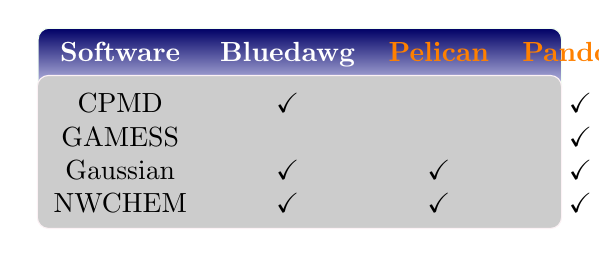
\begin{tikzpicture}
	\node (tbl) {
	\begin{tabularx}{0.55\textwidth}{cccc}
	  \arrayrulecolor{tigersgold}
	  \textcolor{white}{\textbf{Software}} & \textcolor{white}{\textbf{Bluedawg}} & \textcolor{orange}{\textbf{Pelican}} & \textcolor{orange}{\textbf{Pandora}}\\
	  CPMD\rule{0pt}{3.5ex} & \checkmark &  & \checkmark\\
	  GAMESS &  &  & \checkmark\\
	  Gaussian & \checkmark & \checkmark & \checkmark\\
	  NWCHEM & \checkmark & \checkmark & \checkmark \\
	  [1.0ex]
	\end{tabularx}};
	\begin{pgfonlayer}{background}
	  \draw[rounded corners,top color=blue!40!black,bottom color=blue!10!white,draw=green!5!white] ($(tbl.north west)+(0.14,0)$) rectangle ($(tbl.north east)-(0.13,0.9)$);
	  \draw[rounded corners,top color=black!20!white,bottom color=black!20!white,draw=purple!5] ($(tbl.north east)-(0.13,0.6)$) rectangle ($(tbl.south west)+(0.13,0.2)$);
	\end{pgfonlayer}
      \end{tikzpicture}
    \end{center}
  \end{columns}
  }
\end{frame}

\begin{frame}
  \frametitle{\small Computational Chemistry Programs}
  \begin{itemize}
    \item {\color{black}Commercial Software: Q-Chem, Jaguar,CHARMM}
    \item {\color{tigerspurple}GPL/Free Software: ACES, ABINIT, Octopus}
    \item {\color{tigersblue}{\bf \url{http://en.wikipedia.org/wiki/Quantum\_chemistry\_computer\_programs}}}
    \item {\color{tigersblue}{\bf \url{http://www.ccl.net/chemistry/links/software/index.shtml}}}
    \item {\color{tigersblue}{\bf \url{http://www.redbrick.dcu.ie/~noel/linux4chemistry/}}}
  \end{itemize}
\end{frame}

\begin{frame}
  \frametitle{\small Job Types and Keywords}
  \vspace{-0.5cm}
  \begin{columns}
    \column{12cm}
    \begin{block}{}
      \begin{tabular}{|c|c|c|c|}
	\hline
	Job Type & Gaussian & GAMESS & NWCHEM\\
	\cline{2-4}
	& \# keyword & runtyp= & task \\       
	\hline
	Energy & sp & energy & energy \\
	Force & force & gradient & gradient \\
	Geometry optimization & opt & optimize & optimize \\
	Transition State & opt=ts & sadpoint & saddle \\
	Frequency & freq & hessian & frequencies, freq \\
	Potential Energy Scan & scan & surface & \checkmark \\
	Excited State & \checkmark & \checkmark & \checkmark \\
	Reaction path following & irc & irc & \checkmark \\
	Molecular Dynamics & admp, bomd & drc & dynamics, Car-Parrinello \\
	Population Analysis & pop & pop & \checkmark \\
	Electrostatic Properties & prop & \checkmark & \checkmark \\
	Molecular Mechanics & \checkmark & \checkmark & \checkmark \\
	Solvation Models & \checkmark & \checkmark & \checkmark \\
	QM/MM & oniom & \checkmark & qmmm \\
	\hline
      \end{tabular}
    \end{block}
  \end{columns}
\end{frame}

\begin{frame}
  \frametitle{\small Using Gaussian on LONI/LSU HPC Systems}
  \begin{eblock}{}
  \begin{itemize}
    \item Site specific license% ({\color{tigerspurple}Gaussian 03})
    \begin{enumerate}
      \item {\color{tigersblue}Gaussian 03 and 09}
      \begin{itemize}
	\item {\color{tigersblue}LSU Users}: Eric, {\color{green!30!black}Pandora, Pelican, Philip, Tezpur}
	\item {\color{tigersblue}Latech Users}: Painter, Bluedawg
      \end{itemize}
      \item {\color{tigerspurple}Gaussian 03}
      \begin{itemize}
	\item {\color{tigerspurple}ULL Users}: Oliver, \sout{Zeke}
	\item {\color{tigerspurple}Tulane Users}: Louie, \sout{Ducky}
	\item {\color{tigerspurple}Southern Users}: \sout{Lacumba}
      \end{itemize}
      \item UNO Users: No License
    \end{enumerate}
    \item Add {\texttt +gaussian-03/+gaussian-09} to your .soft file and resoft
    \item \alert{If your institution has license to both G03 and G09, have only one active at a given time.}
    \item \alert{Only LSU has a LINDA license to run Gaussian on multiple nodes.}
  \end{itemize}
  \end{eblock}
\end{frame}

\begin{frame}
  \frametitle{\small Input Files}
  \begin{itemize}
    \item Input files for GAMESS, GAUSSIAN and NWCHEM are written in free format.
    \item Molecule description in either Z-Matrix format or Cartesian Coordinates.
    \item Gaussian: Need to specify number of processors to be used in input file \texttt{\%NProcShared}
  \end{itemize}
\end{frame}

\begin{frame}
  \begin{columns}
    \column{8.5cm}
    \vspace{-0.5cm}
    \begin{eblock}{Gaussian Input: h2o-opt-freq.com}
      \begin{tabular}{lcr}
	\%chk=h2o-opt-freq.chk   & & {\color{red}checkpoint file} \\
	\%mem=512mb              & & {\color{red}amount of memory} \\
	\%NProcShared=4          & & {\color{red}number of smp processors} \\
				 & & {\color{red}blank line} \\
	\#p b3lyp/6-31G opt freq & & {\color{red}Job description} \\
				 & & {\color{red}blank line} \\
	H2O OPT FREQ B3LYP       & & {\color{red}Job Title} \\
				 & & {\color{red}blank line} \\
	0 1                      & & {\color{red}Charge \& Multiplicity} \\
	O                        & & {\color{red}Molecule Description} \\
	H 1 r1                   & & {\color{red}in Z-matrix format} \\
	H 1 r1 2 a1              & & {\color{red}with variables} \\
				 & & {\color{red}blank line} \\
	r1 1.05                  & & {\color{red}variable value} \\
	a1 104.5                 & & {\color{red}} \\
				 & & {\color{red}blank line} \\
      \end{tabular}
    \end{eblock}
  \end{columns}
\end{frame}

\begin{frame}
  \frametitle{\small Submission Script for Gaussian}
  \begin{eblock}{}
    \begin{tabular}{l}
      \#!/bin/tcsh\\
      \#PBS -q checkpt \\
      \#PBS -l nodes=1:ppn=4\\
      \#PBS -l walltime=24:00:00\\
      \#PBS -o g09\_testjobs.out\\
      \#PBS -j oe\\
      \#PBS -V \\
      \#PBS -N h2o-opt-freq\\
      \\
      setenv WORK\_DIR \$PBS\_O\_WORKDIR\\
      cd \$WORK\_DIR\\
      setenv OMP\_NUM\_THREADS 4\\
      set NPROCS=`wc -l \$PBS\_NODEFILE |gawk '//{print \$1}'`\\
      \\
      g09 < h2o-opt-freq.com > h2o-opt-freq.log
      \\
    \end{tabular}
  \end{eblock}
\end{frame}

\begin{frame}
  \begin{columns}
    \column{11cm}
    \begin{eblock}{GAMESS Input: h2o-opt-freq.inp}
      {\scriptsize
      \begin{tabular}{lr}
	\$CONTRL SCFTYP=RHF RUNTYP=OPTIMIZE       & {\color{red}Job Control Data} \\
	\quad COORD=ZMT NZVAR=0 \$END             & {\color{red}} \\
	\$STATPT OPTTOL=1.0E-5 HSSEND=.T. \$END   & {\color{red}Geometry Search Control} \\
	\$BASIS GBASIS=N31 NGAUSS=6               & {\color{red}Basis Set} \\
	\quad NDFUNC=1 NPFUNC=1 \$END             & {\color{red}} \\
	\$DATA                                    & {\color{red}Molecular Data Control} \\
	H2O OPT                                   & {\color{red}Job Title} \\
	Cnv 2                                     & {\color{red}Molecule Symmetry group and axis} \\
						  & {\color{red}} \\
	O                                         & {\color{red}Molecule Description} \\
	H 1 rOH                                   & {\color{red}in Z-Matrix} \\
	H 1 rOH 2 aHOH                            & {\color{red}} \\
						  & {\color{red}} \\
	rOH=1.05                                  & {\color{red}Variables} \\
	aHOH=104.5                                & {\color{red}} \\
	\$END                                     & {\color{red}End Molecular Data Control} \\
      \end{tabular}
      }
    \end{eblock}
  \end{columns}
\end{frame}

\begin{frame}
  \frametitle{\small Submission Script for GAMESS}
  \begin{eblock}{}
    \begin{tabular}{l}
      \#!/bin/bash\\
      \#PBS -q checkpt\\
      \#PBS -l nodes=1:ppn=4\\
      \#PBS -l walltime=01:00:00\\
      \#PBS -V\\
      \#PBS -j oe\\
      \#PBS -o gamess-water.out\\
      \#PBS -N gamess-exam1\\
      \\
      export WORKDIR=\$PBS\_O\_WORKDIR\\
      export NPROCS=`wc -l \$PBS\_NODEFILE | gawk '//{print \$1}'`\\
      export SCRDIR=/work/\$USER/scr/\\
      if [ ! -e \$SCRDIR ]; then mkdir -p \$SCRDIR; fi\\
      rm -f \$SCRDIR/*\\
      \\
      cd \$PBS\_O\_WORKDIR\\
      rungms h2o-opt-freq 01 \$NPROCS h2o-opt-freq.out \$SCRDIR\\
      \\      
    \end{tabular}
  \end{eblock}
\end{frame}

\begin{frame}
  \begin{columns}
    \column{5.5cm}
    {\tiny
    \begin{eblock}{NWCHEM Input: h2o-opt-freq.nw}
      \begin{tabular}{lr}
	title "H2O"            & {\color{red}Job title} \\
	echo                   & {\color{red}echo contents of input file} \\
	charge 0               & {\color{red}charge of molecule} \\
	geometry               & {\color{red}geometry description in} \\
	\quad zmatrix          & {\color{red}z-matrix format} \\
	\quad\quad O           & {\color{red}} \\
	\quad\quad H 1 r1      & {\color{red}} \\
	\quad\quad H 1 r1 2 a1 & {\color{red}} \\
	\quad variables        & {\color{red}variables used with values} \\
	\quad\quad r1 1.05     & {\color{red}} \\
	\quad\quad a1 104.5    & {\color{red}} \\
	\quad end              & {\color{red}end z-matrix block} \\
	end                    & {\color{red}end geometry block} \\
	basis noprint          & {\color{red}basis description} \\
	\quad * library 6-31G  & {\color{red}} \\
	end                    & {\color{red}} \\
	dft                    & {\color{red}dft calculation options} \\
	\quad XC b3lyp         & {\color{red}} \\
	\quad mult 1           & {\color{red}} \\
	end                    & {\color{red}} \\
	task dft optimize      & {\color{red}job type: geometry optimization} \\
	task dft energy        & {\color{red}job type: energy calculation} \\
	task dft freq          & {\color{red}job type: frequency calculation} \\
      \end{tabular}
    \end{eblock}
    }
  \end{columns}
\end{frame}

\begin{frame}
  \frametitle{\small Submission Script for NWChem}
  \vspace{-0.3cm}
  \begin{eblock}{}
    \begin{tabular}{l}
      \#!/bin/bash\\
      \#PBS -q checkpt\\
      \#PBS -l nodes=1:ppn=4\\
      \#PBS -l walltime=0:30:00\\
      \#PBS -V\\
      \#PBS -o nwchem\_h2o.out\\
      \#PBS -e nwchem\_h2o.err\\
      \#PBS -N nwchem\_h2o \\
      \\
      export EXEC=nwchem\\
      export EXEC\_DIR=/usr/local/packages/ \textbackslash \\
	\quad nwchem-5.1-mvapich-1.0-intel-10.1/bin/LINUX64/\\
      export WORK\_DIR=\$PBS\_O\_WORKDIR\\
      export NPROCS=`wc -l \$PBS\_NODEFILE |gawk '//{print \$1}'` \\
      \\
      cd \$WORK\_DIR\\
      mpirun\_rsh -machinefile \$PBS\_NODEFILE -np \$NPROCS \textbackslash \\
	\quad \$EXEC\_DIR/\$EXEC \$WORK\_DIR/h2o-opt-freq.nw >\& \textbackslash \\
	\quad \$WORK\_DIR/h2o-opt-freq.nwo\\
      \\
    \end{tabular}
  \end{eblock}
\end{frame}

\section{Exercises}
\begin{frame}
  \frametitle{\small Exercises}
  {\scriptsize
  \begin{exampleblock}{Goals}
    \begin{itemize}
      \item Create Gaussian (or GAMESS/NWChem) Input files for 
      \begin{enumerate}
	{\scriptsize
	\item Optimization
	\item Scan: relaxed and optimized
	\item Properties: Electrostatics, MOs, etc
	\item AIMD
	}
      \end{enumerate}
    \end{itemize}
  \end{exampleblock}
  \begin{block}{Assignment}
    \begin{itemize}
      \item Molecule: $[NH_3-H-NH_3]^+$
      \item Method/Basis: B3LYP/6-311++G(D,P)
      \item Job Type: Geometry Optimization + Freqeuncy
      \item Scan along the $N-H-N$ axis by moving the $H$, bonded to one $N$ to the other and analyze and discuss  the Potential Energy Curve.
      \item Population Analysis: Calculate and visualize MO's and electrostatic potential around the molecule.
      \item Optional: Run an AIMD simulation for at least 2ps and obtain a spectra. Compare with the harmonic spectra.
    \end{itemize}
  \end{block}
  }
\end{frame}

\section{Tips for Quantum Chemical Calculations}
\begin{frame}
  \frametitle{\small Choosing Basis Sets}
%\frametitle{\small Basis Sets and Method}\vspace{1cm}
% \vspace{0.5cm}
  \begin{colorblock}{white}{blue!30!black}{black}{white!80!black}{Choice of Basis Set}
    \begin{itemize}
      \item STO-3G is too small.
      \item 6-31G* and 6-31G** give reasonable results.
      \item For greater accuracy, use correlation consistent basis sets e.g. cc-pVTZ
      \item For anions and probably excited states, use basis sets with diffuse functions (aug, +). e.g. 6-31+G*, aug-cc-pVTZ
    \end{itemize}
  \end{colorblock}
  \vspace{0.5cm}
  \begin{colorblock}{white}{blue!30!black}{black}{white!80!black}{GAMESS Basis Sets}
    \begin{itemize}
      \item In GAMESS, you can create a file containing basis sets that you want to use
      \item Define \texttt{EXTBAS} variable which points to the basis set file
      \item See pseudo basis example
      \item In input line, if you name your basis set as \texttt{STTGRD}, then add
      \texttt{\$BASIS EXTFIL=.T. GBASIS=STTGRD \$END}
    \end{itemize}
  \end{colorblock}
\end{frame}

\begin{frame}
  \frametitle{\small Method and SCF Convergence}
  \vspace{-0.2cm}
  \begin{colorblock}{white}{blue!30!black}{black}{white!80!black}{Choice of Method}
    \begin{itemize}
      \item Always pick DFT over HF
      \item In general: HF < DFT $\sim$ MP2 < CCSD < CCSD(T)
      \item Pay attention to scaling behavior
    \end{itemize}
  \end{colorblock}
% \vspace{0.5cm}
  \begin{colorblock}{white}{blue!30!black}{black}{white!80!black}{SCF Convergence Issues}
    \begin{itemize}
      \item Has SCF (HF and DFT) really converged? Important if you use iop(5/13) in Gaussian route card.
      \item If SCF doesn't converge:
      \begin{enumerate}
	{\footnotesize
	\item Increase maximum number of SCF iterations.
	\begin{itemize}
	  {\footnotesize
	  \item GAMESS: max 200 SCF iterations cannot be increased further.}
	\end{itemize}
	\item Use smaller basis set as an initial guess.
	\item Try level shifting
	\item Use forced convergence method:
	\begin{itemize}
	  {\footnotesize
	  \item Gaussian: SCF=QC, XQC or DM and item 1 above
	  \item GAMESS: SOSCF}
	\end{itemize}
	}
      \end{enumerate}
    \end{itemize}
  \end{colorblock}
\end{frame}

\begin{frame}
  \frametitle{\small Geometry Optimizations}
  \begin{colorblock}{white}{blue!30!black}{black}{white!80!black}{Geometry Optimizations}
    \begin{itemize}
      \item Many problems in computational chemistry are optimization problems: i.e., finding the "stationary points" where a multidimensional function has vanishing gradients.
      \item The energy as a function of nuclear coordinates. Minima, transition states may be of interest.
      \item Make sure that the geometry optimization actually converges.
      \item Run a frequency calculation to check whether the geometry is a local minima (zero imaginary frequencies) or a transition state (only one imaginary frequency)
      \item Tighten convergence criterion to remove unwanted imaginary frequencies.
      \item Having more than 3N-6 (3N-5 for linear) frequencies implies that you are not at a minimum. Double check and tighten convergence if necessary.
    \end{itemize}
  \end{colorblock}
\end{frame}

\begin{frame}
  \frametitle{\small Worked out Examples On LONI Linux Systems}
  \begin{columns}
    \column{1.16\textwidth}
    \vspace{-0.95cm}
    \begin{alertblock}{On LONI Linux Systems}
      \begin{center}
	\includegraphics[width=0.63\textwidth,clip=true]{workshop}
      \end{center}
    \end{alertblock}
  \end{columns}
\end{frame}

\begin{frame}
\frametitle{\small Useful Links/Further Reading}
  \vspace{-0.25cm}
  \begin{block}{Useful Links}
    \begin{itemize}
      {\tiny
      \item {\color{tigerspurple}GAMESS:} {\color{Blue}\url{http://www.msg.chem.iastate.edu/gamess}}
      \item {\color{tigerspurple}Gaussian:} {\color{Blue}\url{http://www.gaussian.com}}
      \item {\color{tigerspurple}NWCHEM:} {\color{Blue}\url{http://www.nwchem-sw.org}}
      \item {\color{tigerspurple}Basis Set:} {\color{Blue}\url{https://bse.pnl.gov/bse/portal}}
      }
    \end{itemize}
  \end{block}
  \vspace{-0.2cm}
  \begin{block}{\small Further Reading}
    \begin{itemize}
      {\tiny
      \item David Sherill's Notes at Ga Tech: {\color{Blue}\url{http://vergil.chemistry.gatech.edu/notes/index.html}}
      \item David Young's Notes on CCL: {\color{Blue}\url{http://www.ccl.net/cca/documents/dyoung/}}
      \item Mark Tuckerman's Notes at NYU: {\color{Blue}\url{http://www.nyu.edu/classes/tuckerman/quant.mech/index.html}}
      \item Modern Quantum Chemistry: Introduction to Advanced Electronic Structure Theory, A. Szabo and N. Ostlund
      \item Introduction to Computational Chemistry, F. Jensen
      \item Essentials of Computational Chemistry - Theories and Models, C. J. Cramer
      \item Exploring Chemistry with Electronic Structure Methods, J. B. Foresman and A. Frisch
%\item Ab Initio Molecular Dynamics: Theory and Implementation, D. Marx and J. Hutter{\color{Blue}\url{http://www.theochem.ruhr-uni-bochum.de/research/marx/marx.pdf}}
%\item Molecular Modeling - Principles and Applications, A. R. Leach
%\item Computer Simulation of Liquids, M. P. Allen and D. J. Tildesley
      \item[$\vardiamond$]Modern Electronic Structure Theory, T. Helgaker, P. Jorgensen and J. Olsen (Highly advanced text, second quantization approach to electronic structure theory)
      }
    \end{itemize}
  \end{block}
\end{frame}

\end{document}

